\documentclass{article}
\usepackage{amsmath}
\usepackage{pgfplots}
\usepackage{verbatim}
\usepackage{tikz}
\pgfplotsset{compat=1.18}


\title{Physics informed neural network of a moving conductive string in a magnetic field}
\author{Jalil Hasanyan}
\date{\today}

\begin{document}

\maketitle

\section{Physical Model}
Consider an infinite conductive string an a homogeneous magnetic field, $\textbf{B}_0 = B_0 \textbf{i}_x$, where $B_0$ is a constant. The string is being pulled at a constant velocity, $\textbf{V} = V_0 \textbf{i}_x$, through two rings which are located a distance $l$ from each other. The motion of the string is considered in a fixed Cartesian coordinate system $(x,y,z)$, with unit vectors $\textbf{i}_x, \textbf{i}_y, \textbf{i}_z$. The center of one of the rings is assumed to be the center of the coordinate system.

\begin{figure}[ht]
\centering
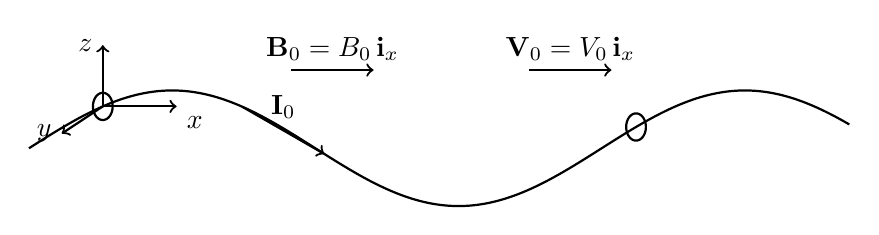
\begin{tikzpicture}

\begin{axis}[
  width=12cm,
  height=4cm,
  axis lines=none,
  xmin=0, xmax=10,
  ymin=-1.4, ymax=1.4,
  clip=false
]

% Wavy string
\addplot[thick, smooth, samples=200, domain=0:10]
  {0.85*sin(deg(0.9*x))};

% --- Define left loop location ---
\pgfmathsetmacro{\xloop}{0.9}
\pgfmathsetmacro{\yloop}{0.85*sin(deg(0.9*\xloop))}

% Precompute axis-coordinate endpoints for the triad
\pgfmathsetmacro{\xplus}{\xloop + 0.9}
\pgfmathsetmacro{\xminus}{\xloop - 0.5}
\pgfmathsetmacro{\yminus}{\yloop - 0.4}
\pgfmathsetmacro{\yplus}{\yloop + 0.9}

% --- Coordinate triad attached to left loop ---
\draw[->,thick] (axis cs:\xloop,\yloop) -- (axis cs:\xplus,\yloop)
  node[below right] {$x$};
\draw[->,thick] (axis cs:\xloop,\yloop) -- (axis cs:\xminus,\yminus)
  node[left] {$y$};
\draw[->,thick] (axis cs:\xloop,\yloop) -- (axis cs:\xloop,\yplus)
  node[left] {$z$};

% --- Left loop ---
\addplot[thick, domain=0:360, samples=100]
  ({\xloop + 0.12*cos(x)}, {\yloop + 0.20*sin(x)});

% --- Right loop (new) ---
\pgfmathsetmacro{\xloopR}{7.4}
\pgfmathsetmacro{\yloopR}{0.85*sin(deg(0.9*\xloopR))}
\addplot[thick, domain=0:360, samples=100]
  ({\xloopR + 0.12*cos(x)}, {\yloopR + 0.20*sin(x)});

% B0 arrow
\draw[->,thick] (axis cs:3.2,1.15) -- (axis cs:4.2,1.15);
\node[above] at (axis cs:3.7,1.15) {$\mathbf{B}_0 = B_0\,\mathbf{i}_x$};

% V0 arrow
\draw[->,thick] (axis cs:6.1,1.15) -- (axis cs:7.1,1.15);
\node[above] at (axis cs:6.6,1.15) {$\mathbf{V}_0 = V_0\,\mathbf{i}_x$};
% --- Current arrow along the string + label on the string (new) ---
% Pick two x-positions along the curve and compute y from the same function
\pgfmathsetmacro{\xIstart}{2.6}
\pgfmathsetmacro{\yIstart}{0.85*sin(deg(0.9*\xIstart))}
\pgfmathsetmacro{\xIend}{3.6}
\pgfmathsetmacro{\yIend}{0.85*sin(deg(0.9*\xIend))}
\pgfmathsetmacro{\xImid}{0.5*(\xIstart+\xIend)}
\pgfmathsetmacro{\yImid}{0.85*sin(deg(0.9*\xImid))}

% Arrow (direction: start -> end)
\draw[->,thick] (axis cs:\xIstart,\yIstart) -- (axis cs:\xIend,\yIend);

% Label placed on/near the curve
\node[above] at (axis cs:\xImid,\yImid) {$\textbf{I}_0$};

\end{axis}
\end{tikzpicture}
\caption{Schematic of the string with the applied fields and forces.}
\label{fig:string_schematic}
\end{figure}


The influence of gravity and other external forces are neglected. The unit length and the position of each material point of the string is assumed to be constant. We identify the position of each material point of the string through its arc length $s \in [0,l]$. In Euclidean space, we denote the displacement of the string by $\textbf{r}(t,s) = x(t,s) \textbf{i}_x + y(t,s) \textbf{i}_y + z(t,s) \textbf{i}_z$. We also assume that $\textbf{k} = \frac{\partial x }{\partial s} \textbf{i}_x + \frac{\partial y }{\partial s} \textbf{i}_y + \frac{\partial z }{\partial s} \textbf{i}_z$ represents the unit vector directed along the tangent to the deformed line of the string. If we assume a current $\textbf{I} = I_0(t) \textbf{k}$ flows through the string, then the magnetic field will exert forces on the string. In this particular case, the forces acting on the string are called Laplace forces given by
\begin{equation}
    \textbf{F} = I_0 B_0 (\textbf{k} \times \textbf{i}_x).
\end{equation}
The motion of the string is described by
\begin{equation}
    \frac{\partial \textbf{Q}}{\partial s} + \textbf{F} = \rho \textbf{R}, \qquad \textbf{Q} \times \textbf{k} = 0, \qquad \big( \frac{\partial \textbf{r}}{\partial s} \big) = 1,
\end{equation}
where $\textbf{Q}$ is the internal tension in the string, $\rho$ is the mass density per unit length, and $\textbf{R}$ is the acceleration of the string given by
\begin{equation}
    R_x = 0, \qquad R_y = \frac{\partial^2 y}{\partial t^2} + 2V_0 \frac{\partial^2 y}{\partial s \partial t} + V_0^2 \frac{\partial^2 y}{\partial s^2} + \eta \frac{\partial y}{\partial t}, \qquad R_z = \frac{\partial^2 z}{\partial t^2} + 2V_0 \frac{\partial^2 z}{\partial s \partial t} + V_0^2 \frac{\partial^2 z}{\partial s^2}+ \eta \frac{\partial z}{\partial t}.
\end{equation}



The motion of the string generates an induced electric field due to the relative motion of the conductor in the magnetic field. This setup is governed by Faraday's law of induction and the Lorentz force law. The resulting electric field is proportional to the velocity of the string and the strength of the magnetic field. The system is modeled using a set of partial differential equations that describe both the electromagnetic and mechanical behavior of the string.






\begin{comment}
Here is an equation:
\[
E = mc^2
\]

\begin{center}
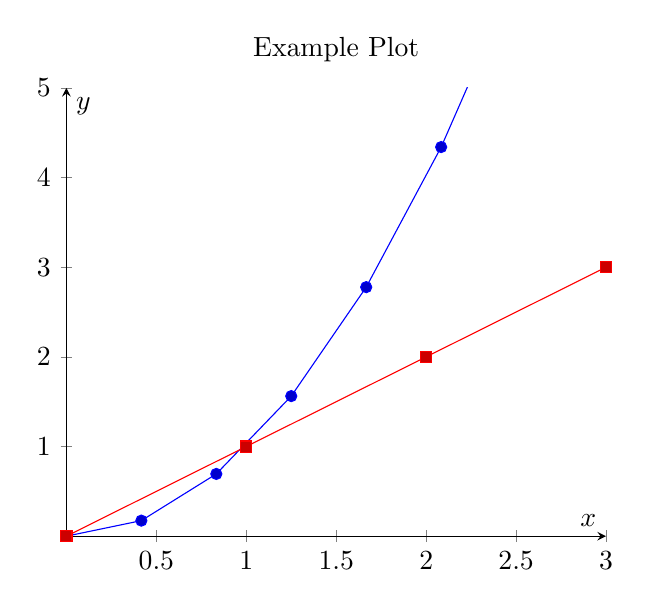
\begin{tikzpicture}
\begin{axis}[
    xmin=0, xmax=3,
    ymin=0, ymax=5, 
    xlabel=$x$,
    ylabel=$y$,
    title={Example Plot}, 
    axis lines=middle]
\addplot{x^2};
\addplot coordinates {(0,0) (1,1) (2,2) (3,3)};
\end{axis}
\end{tikzpicture}
\end{center}
\end{comment}




\end{document}
